\section{Exercise 4: Dale's law}

\begin{itshape}
\small
Set $c=0.1$, $N = 200$ and turn off random asymmetry ($p_{cut} = 0$). Set $E \in \l[0, 1\r]$ to be the percentage of excitatory nodes.

For a given $E$, randomly split the network into an excitatory and an inhibitory subpopulation (of sizes $E \cdot N$ and $(1 - E) \cdot N$ respectively). Now enforce Dale's law on the network connectivity by setting '"disallowed"` connection weights in the standard Hebbian weight matrix Eq. 1 to zero.

What percentage of the directed connections do you expect to be cut for $E = \frac{1}{2}$
As in Ex. 2 calculate and plot the mean $\alpha_{N,max}$ for varying E with error bars (at least 10 repetitions). Interpret the results and compare the value for E = 1 to your result from Ex. 3.
\end{itshape}

\paragraph*{}

\begin{wrapfigure}{r}{0.5\textwidth}
  \vspace{-20pt}
  \begin{center}
%    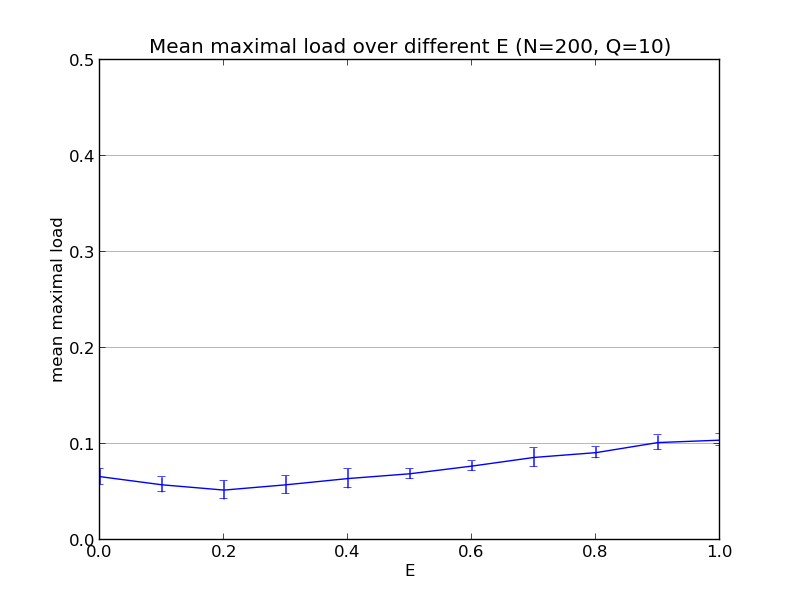
\includegraphics[width=0.6\textwidth]{dat/ex4-mean_max_load-N200-Q10-C95.png}
  \end{center}
  \vspace{-20pt}
  \caption{Exercise 4: Mean maximal load over different E}
  \label{fig: Question 1.3}
  \vspace{-10pt}
\end{wrapfigure}


